% Created by tikzDevice version 0.12.3.1 on 2021-06-16 15:27:59
% !TEX encoding = UTF-8 Unicode
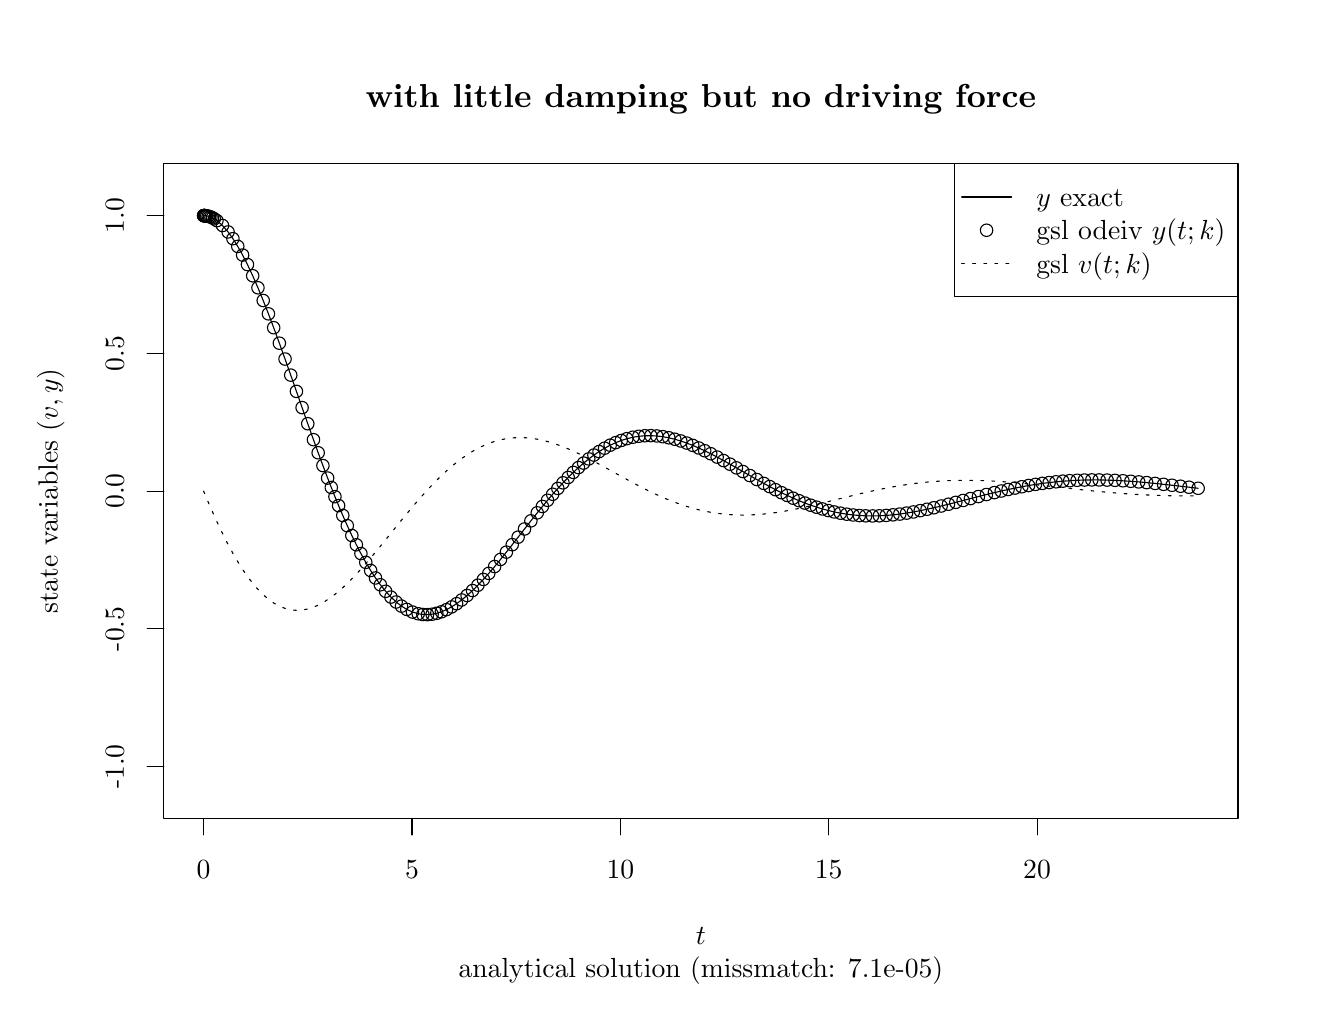
\begin{tikzpicture}[x=1pt,y=1pt]
\definecolor{fillColor}{RGB}{255,255,255}
\path[use as bounding box,fill=fillColor,fill opacity=0.00] (0,0) rectangle (462.53,346.90);
\begin{scope}
\path[clip] ( 49.20, 61.20) rectangle (437.33,297.70);
\definecolor{drawColor}{RGB}{0,0,0}

\path[draw=drawColor,line width= 0.4pt,line join=round,line cap=round] ( 63.58,278.98) --
	( 63.60,278.98) --
	( 63.66,278.98) --
	( 63.72,278.98) --
	( 63.78,278.98) --
	( 63.84,278.98) --
	( 63.89,278.98) --
	( 63.95,278.97) --
	( 64.03,278.97) --
	( 64.17,278.96) --
	( 64.39,278.93) --
	( 64.75,278.87) --
	( 65.24,278.76) --
	( 65.73,278.61) --
	( 66.23,278.43) --
	( 66.76,278.18) --
	( 67.42,277.82) --
	( 68.40,277.17) --
	( 70.41,275.40) --
	( 72.42,273.09) --
	( 74.17,270.65) --
	( 75.92,267.86) --
	( 77.67,264.73) --
	( 79.42,261.29) --
	( 81.31,257.25) --
	( 83.21,252.91) --
	( 85.11,248.31) --
	( 87.00,243.49) --
	( 88.90,238.48) --
	( 90.95,232.89) --
	( 93.00,227.16) --
	( 95.06,221.35) --
	( 97.11,215.49) --
	( 99.16,209.62) --
	(101.21,203.78) --
	(103.27,198.02) --
	(104.97,193.30) --
	(106.68,188.67) --
	(108.39,184.16) --
	(109.71,180.76) --
	(111.03,177.44) --
	(112.35,174.21) --
	(113.86,170.66) --
	(115.49,166.95) --
	(117.13,163.41) --
	(118.77,160.05) --
	(120.41,156.88) --
	(122.17,153.70) --
	(123.93,150.76) --
	(125.68,148.06) --
	(127.44,145.61) --
	(129.35,143.23) --
	(131.26,141.15) --
	(133.16,139.37) --
	(135.07,137.89) --
	(136.98,136.71) --
	(139.05,135.75) --
	(141.12,135.13) --
	(142.80,134.87) --
	(144.48,134.81) --
	(146.15,134.96) --
	(147.83,135.30) --
	(149.51,135.83) --
	(151.33,136.61) --
	(153.16,137.59) --
	(154.99,138.76) --
	(156.82,140.10) --
	(158.78,141.72) --
	(160.74,143.51) --
	(162.70,145.45) --
	(164.66,147.52) --
	(166.62,149.71) --
	(168.74,152.18) --
	(170.86,154.75) --
	(172.98,157.39) --
	(175.10,160.08) --
	(177.22,162.79) --
	(179.53,165.74) --
	(181.83,168.68) --
	(184.13,171.57) --
	(185.99,173.87) --
	(187.85,176.11) --
	(189.71,178.29) --
	(191.57,180.39) --
	(193.43,182.42) --
	(195.30,184.35) --
	(197.16,186.19) --
	(199.02,187.92) --
	(200.88,189.54) --
	(202.74,191.05) --
	(204.60,192.44) --
	(206.46,193.71) --
	(208.47,194.93) --
	(210.48,196.01) --
	(212.49,196.94) --
	(214.49,197.73) --
	(216.50,198.36) --
	(218.67,198.88) --
	(220.83,199.24) --
	(223.00,199.43) --
	(225.16,199.46) --
	(227.33,199.35) --
	(229.49,199.09) --
	(231.66,198.70) --
	(233.83,198.18) --
	(235.99,197.54) --
	(238.16,196.79) --
	(240.32,195.95) --
	(242.49,195.02) --
	(244.65,194.01) --
	(246.82,192.94) --
	(249.14,191.73) --
	(251.46,190.47) --
	(253.78,189.17) --
	(256.10,187.85) --
	(258.43,186.51) --
	(260.94,185.07) --
	(263.46,183.63) --
	(265.98,182.23) --
	(268.10,181.08) --
	(270.22,179.96) --
	(272.34,178.89) --
	(274.46,177.87) --
	(276.58,176.90) --
	(278.70,175.98) --
	(280.82,175.13) --
	(282.94,174.35) --
	(285.06,173.63) --
	(287.18,172.99) --
	(289.30,172.42) --
	(291.42,171.92) --
	(293.70,171.47) --
	(295.98,171.10) --
	(298.26,170.82) --
	(300.54,170.62) --
	(302.82,170.51) --
	(305.29,170.47) --
	(307.75,170.52) --
	(310.21,170.65) --
	(312.67,170.86) --
	(315.13,171.15) --
	(317.59,171.50) --
	(320.05,171.91) --
	(322.52,172.37) --
	(324.98,172.88) --
	(327.44,173.42) --
	(330.08,174.05) --
	(332.73,174.70) --
	(335.37,175.36) --
	(338.02,176.04) --
	(340.66,176.73) --
	(343.55,177.47) --
	(346.43,178.19) --
	(349.32,178.89) --
	(351.79,179.46) --
	(354.27,180.01) --
	(356.74,180.52) --
	(359.22,181.00) --
	(361.69,181.45) --
	(364.16,181.85) --
	(366.64,182.21) --
	(369.11,182.52) --
	(371.59,182.79) --
	(374.06,183.02) --
	(376.54,183.19) --
	(379.20,183.34) --
	(381.86,183.43) --
	(384.52,183.47) --
	(387.18,183.47) --
	(390.04,183.41) --
	(392.90,183.31) --
	(395.76,183.16) --
	(398.61,182.98) --
	(401.47,182.76) --
	(404.33,182.50) --
	(407.39,182.21) --
	(410.45,181.88) --
	(413.52,181.55) --
	(416.58,181.20) --
	(419.64,180.84) --
	(422.95,180.46);
\end{scope}
\begin{scope}
\path[clip] (  0.00,  0.00) rectangle (462.53,346.90);
\definecolor{drawColor}{RGB}{0,0,0}

\path[draw=drawColor,line width= 0.4pt,line join=round,line cap=round] ( 63.58, 61.20) -- (364.75, 61.20);

\path[draw=drawColor,line width= 0.4pt,line join=round,line cap=round] ( 63.58, 61.20) -- ( 63.58, 55.20);

\path[draw=drawColor,line width= 0.4pt,line join=round,line cap=round] (138.87, 61.20) -- (138.87, 55.20);

\path[draw=drawColor,line width= 0.4pt,line join=round,line cap=round] (214.16, 61.20) -- (214.16, 55.20);

\path[draw=drawColor,line width= 0.4pt,line join=round,line cap=round] (289.46, 61.20) -- (289.46, 55.20);

\path[draw=drawColor,line width= 0.4pt,line join=round,line cap=round] (364.75, 61.20) -- (364.75, 55.20);

\node[text=drawColor,anchor=base,inner sep=0pt, outer sep=0pt, scale=  1.00] at ( 63.58, 39.60) {0};

\node[text=drawColor,anchor=base,inner sep=0pt, outer sep=0pt, scale=  1.00] at (138.87, 39.60) {5};

\node[text=drawColor,anchor=base,inner sep=0pt, outer sep=0pt, scale=  1.00] at (214.16, 39.60) {10};

\node[text=drawColor,anchor=base,inner sep=0pt, outer sep=0pt, scale=  1.00] at (289.46, 39.60) {15};

\node[text=drawColor,anchor=base,inner sep=0pt, outer sep=0pt, scale=  1.00] at (364.75, 39.60) {20};

\path[draw=drawColor,line width= 0.4pt,line join=round,line cap=round] ( 49.20, 79.91) -- ( 49.20,278.98);

\path[draw=drawColor,line width= 0.4pt,line join=round,line cap=round] ( 49.20, 79.91) -- ( 43.20, 79.91);

\path[draw=drawColor,line width= 0.4pt,line join=round,line cap=round] ( 49.20,129.68) -- ( 43.20,129.68);

\path[draw=drawColor,line width= 0.4pt,line join=round,line cap=round] ( 49.20,179.45) -- ( 43.20,179.45);

\path[draw=drawColor,line width= 0.4pt,line join=round,line cap=round] ( 49.20,229.22) -- ( 43.20,229.22);

\path[draw=drawColor,line width= 0.4pt,line join=round,line cap=round] ( 49.20,278.98) -- ( 43.20,278.98);

\node[text=drawColor,rotate= 90.00,anchor=base,inner sep=0pt, outer sep=0pt, scale=  1.00] at ( 34.80, 79.91) {-1.0};

\node[text=drawColor,rotate= 90.00,anchor=base,inner sep=0pt, outer sep=0pt, scale=  1.00] at ( 34.80,129.68) {-0.5};

\node[text=drawColor,rotate= 90.00,anchor=base,inner sep=0pt, outer sep=0pt, scale=  1.00] at ( 34.80,179.45) {0.0};

\node[text=drawColor,rotate= 90.00,anchor=base,inner sep=0pt, outer sep=0pt, scale=  1.00] at ( 34.80,229.22) {0.5};

\node[text=drawColor,rotate= 90.00,anchor=base,inner sep=0pt, outer sep=0pt, scale=  1.00] at ( 34.80,278.98) {1.0};

\path[draw=drawColor,line width= 0.4pt,line join=round,line cap=round] ( 49.20, 61.20) --
	(437.33, 61.20) --
	(437.33,297.70) --
	( 49.20,297.70) --
	( 49.20, 61.20);
\end{scope}
\begin{scope}
\path[clip] (  0.00,  0.00) rectangle (462.53,346.90);
\definecolor{drawColor}{RGB}{0,0,0}

\node[text=drawColor,anchor=base,inner sep=0pt, outer sep=0pt, scale=  1.20] at (243.26,318.16) {\bfseries  with little damping but no driving force};

\node[text=drawColor,anchor=base,inner sep=0pt, outer sep=0pt, scale=  1.00] at (243.26,  3.60) {analytical solution (missmatch: 7.1e-05)};

\node[text=drawColor,anchor=base,inner sep=0pt, outer sep=0pt, scale=  1.00] at (243.26, 15.60) {$t$};

\node[text=drawColor,rotate= 90.00,anchor=base,inner sep=0pt, outer sep=0pt, scale=  1.00] at ( 10.80,179.45) {state variables $(v,y)$};
\end{scope}
\begin{scope}
\path[clip] ( 49.20, 61.20) rectangle (437.33,297.70);
\definecolor{drawColor}{RGB}{0,0,0}

\path[draw=drawColor,line width= 0.4pt,line join=round,line cap=round] ( 63.58,278.98) circle (  2.25);

\path[draw=drawColor,line width= 0.4pt,line join=round,line cap=round] ( 63.60,278.98) circle (  2.25);

\path[draw=drawColor,line width= 0.4pt,line join=round,line cap=round] ( 63.66,278.98) circle (  2.25);

\path[draw=drawColor,line width= 0.4pt,line join=round,line cap=round] ( 63.72,278.98) circle (  2.25);

\path[draw=drawColor,line width= 0.4pt,line join=round,line cap=round] ( 63.78,278.98) circle (  2.25);

\path[draw=drawColor,line width= 0.4pt,line join=round,line cap=round] ( 63.84,278.98) circle (  2.25);

\path[draw=drawColor,line width= 0.4pt,line join=round,line cap=round] ( 63.89,278.97) circle (  2.25);

\path[draw=drawColor,line width= 0.4pt,line join=round,line cap=round] ( 63.95,278.97) circle (  2.25);

\path[draw=drawColor,line width= 0.4pt,line join=round,line cap=round] ( 64.03,278.96) circle (  2.25);

\path[draw=drawColor,line width= 0.4pt,line join=round,line cap=round] ( 64.17,278.95) circle (  2.25);

\path[draw=drawColor,line width= 0.4pt,line join=round,line cap=round] ( 64.39,278.93) circle (  2.25);

\path[draw=drawColor,line width= 0.4pt,line join=round,line cap=round] ( 64.75,278.87) circle (  2.25);

\path[draw=drawColor,line width= 0.4pt,line join=round,line cap=round] ( 65.24,278.76) circle (  2.25);

\path[draw=drawColor,line width= 0.4pt,line join=round,line cap=round] ( 65.73,278.61) circle (  2.25);

\path[draw=drawColor,line width= 0.4pt,line join=round,line cap=round] ( 66.23,278.43) circle (  2.25);

\path[draw=drawColor,line width= 0.4pt,line join=round,line cap=round] ( 66.76,278.18) circle (  2.25);

\path[draw=drawColor,line width= 0.4pt,line join=round,line cap=round] ( 67.42,277.82) circle (  2.25);

\path[draw=drawColor,line width= 0.4pt,line join=round,line cap=round] ( 68.40,277.16) circle (  2.25);

\path[draw=drawColor,line width= 0.4pt,line join=round,line cap=round] ( 70.41,275.40) circle (  2.25);

\path[draw=drawColor,line width= 0.4pt,line join=round,line cap=round] ( 72.42,273.09) circle (  2.25);

\path[draw=drawColor,line width= 0.4pt,line join=round,line cap=round] ( 74.17,270.65) circle (  2.25);

\path[draw=drawColor,line width= 0.4pt,line join=round,line cap=round] ( 75.92,267.86) circle (  2.25);

\path[draw=drawColor,line width= 0.4pt,line join=round,line cap=round] ( 77.67,264.73) circle (  2.25);

\path[draw=drawColor,line width= 0.4pt,line join=round,line cap=round] ( 79.42,261.30) circle (  2.25);

\path[draw=drawColor,line width= 0.4pt,line join=round,line cap=round] ( 81.31,257.25) circle (  2.25);

\path[draw=drawColor,line width= 0.4pt,line join=round,line cap=round] ( 83.21,252.91) circle (  2.25);

\path[draw=drawColor,line width= 0.4pt,line join=round,line cap=round] ( 85.11,248.31) circle (  2.25);

\path[draw=drawColor,line width= 0.4pt,line join=round,line cap=round] ( 87.00,243.49) circle (  2.25);

\path[draw=drawColor,line width= 0.4pt,line join=round,line cap=round] ( 88.90,238.48) circle (  2.25);

\path[draw=drawColor,line width= 0.4pt,line join=round,line cap=round] ( 90.95,232.89) circle (  2.25);

\path[draw=drawColor,line width= 0.4pt,line join=round,line cap=round] ( 93.00,227.16) circle (  2.25);

\path[draw=drawColor,line width= 0.4pt,line join=round,line cap=round] ( 95.06,221.35) circle (  2.25);

\path[draw=drawColor,line width= 0.4pt,line join=round,line cap=round] ( 97.11,215.48) circle (  2.25);

\path[draw=drawColor,line width= 0.4pt,line join=round,line cap=round] ( 99.16,209.61) circle (  2.25);

\path[draw=drawColor,line width= 0.4pt,line join=round,line cap=round] (101.21,203.78) circle (  2.25);

\path[draw=drawColor,line width= 0.4pt,line join=round,line cap=round] (103.27,198.01) circle (  2.25);

\path[draw=drawColor,line width= 0.4pt,line join=round,line cap=round] (104.97,193.29) circle (  2.25);

\path[draw=drawColor,line width= 0.4pt,line join=round,line cap=round] (106.68,188.67) circle (  2.25);

\path[draw=drawColor,line width= 0.4pt,line join=round,line cap=round] (108.39,184.15) circle (  2.25);

\path[draw=drawColor,line width= 0.4pt,line join=round,line cap=round] (109.71,180.75) circle (  2.25);

\path[draw=drawColor,line width= 0.4pt,line join=round,line cap=round] (111.03,177.43) circle (  2.25);

\path[draw=drawColor,line width= 0.4pt,line join=round,line cap=round] (112.35,174.20) circle (  2.25);

\path[draw=drawColor,line width= 0.4pt,line join=round,line cap=round] (113.86,170.65) circle (  2.25);

\path[draw=drawColor,line width= 0.4pt,line join=round,line cap=round] (115.49,166.94) circle (  2.25);

\path[draw=drawColor,line width= 0.4pt,line join=round,line cap=round] (117.13,163.40) circle (  2.25);

\path[draw=drawColor,line width= 0.4pt,line join=round,line cap=round] (118.77,160.04) circle (  2.25);

\path[draw=drawColor,line width= 0.4pt,line join=round,line cap=round] (120.41,156.87) circle (  2.25);

\path[draw=drawColor,line width= 0.4pt,line join=round,line cap=round] (122.17,153.69) circle (  2.25);

\path[draw=drawColor,line width= 0.4pt,line join=round,line cap=round] (123.93,150.75) circle (  2.25);

\path[draw=drawColor,line width= 0.4pt,line join=round,line cap=round] (125.68,148.05) circle (  2.25);

\path[draw=drawColor,line width= 0.4pt,line join=round,line cap=round] (127.44,145.59) circle (  2.25);

\path[draw=drawColor,line width= 0.4pt,line join=round,line cap=round] (129.35,143.22) circle (  2.25);

\path[draw=drawColor,line width= 0.4pt,line join=round,line cap=round] (131.26,141.14) circle (  2.25);

\path[draw=drawColor,line width= 0.4pt,line join=round,line cap=round] (133.16,139.36) circle (  2.25);

\path[draw=drawColor,line width= 0.4pt,line join=round,line cap=round] (135.07,137.88) circle (  2.25);

\path[draw=drawColor,line width= 0.4pt,line join=round,line cap=round] (136.98,136.69) circle (  2.25);

\path[draw=drawColor,line width= 0.4pt,line join=round,line cap=round] (139.05,135.74) circle (  2.25);

\path[draw=drawColor,line width= 0.4pt,line join=round,line cap=round] (141.12,135.12) circle (  2.25);

\path[draw=drawColor,line width= 0.4pt,line join=round,line cap=round] (142.80,134.85) circle (  2.25);

\path[draw=drawColor,line width= 0.4pt,line join=round,line cap=round] (144.48,134.80) circle (  2.25);

\path[draw=drawColor,line width= 0.4pt,line join=round,line cap=round] (146.15,134.95) circle (  2.25);

\path[draw=drawColor,line width= 0.4pt,line join=round,line cap=round] (147.83,135.29) circle (  2.25);

\path[draw=drawColor,line width= 0.4pt,line join=round,line cap=round] (149.51,135.82) circle (  2.25);

\path[draw=drawColor,line width= 0.4pt,line join=round,line cap=round] (151.33,136.60) circle (  2.25);

\path[draw=drawColor,line width= 0.4pt,line join=round,line cap=round] (153.16,137.59) circle (  2.25);

\path[draw=drawColor,line width= 0.4pt,line join=round,line cap=round] (154.99,138.75) circle (  2.25);

\path[draw=drawColor,line width= 0.4pt,line join=round,line cap=round] (156.82,140.10) circle (  2.25);

\path[draw=drawColor,line width= 0.4pt,line join=round,line cap=round] (158.78,141.72) circle (  2.25);

\path[draw=drawColor,line width= 0.4pt,line join=round,line cap=round] (160.74,143.50) circle (  2.25);

\path[draw=drawColor,line width= 0.4pt,line join=round,line cap=round] (162.70,145.44) circle (  2.25);

\path[draw=drawColor,line width= 0.4pt,line join=round,line cap=round] (164.66,147.52) circle (  2.25);

\path[draw=drawColor,line width= 0.4pt,line join=round,line cap=round] (166.62,149.71) circle (  2.25);

\path[draw=drawColor,line width= 0.4pt,line join=round,line cap=round] (168.74,152.18) circle (  2.25);

\path[draw=drawColor,line width= 0.4pt,line join=round,line cap=round] (170.86,154.75) circle (  2.25);

\path[draw=drawColor,line width= 0.4pt,line join=round,line cap=round] (172.98,157.39) circle (  2.25);

\path[draw=drawColor,line width= 0.4pt,line join=round,line cap=round] (175.10,160.08) circle (  2.25);

\path[draw=drawColor,line width= 0.4pt,line join=round,line cap=round] (177.22,162.80) circle (  2.25);

\path[draw=drawColor,line width= 0.4pt,line join=round,line cap=round] (179.53,165.75) circle (  2.25);

\path[draw=drawColor,line width= 0.4pt,line join=round,line cap=round] (181.83,168.69) circle (  2.25);

\path[draw=drawColor,line width= 0.4pt,line join=round,line cap=round] (184.13,171.58) circle (  2.25);

\path[draw=drawColor,line width= 0.4pt,line join=round,line cap=round] (185.99,173.88) circle (  2.25);

\path[draw=drawColor,line width= 0.4pt,line join=round,line cap=round] (187.85,176.12) circle (  2.25);

\path[draw=drawColor,line width= 0.4pt,line join=round,line cap=round] (189.71,178.30) circle (  2.25);

\path[draw=drawColor,line width= 0.4pt,line join=round,line cap=round] (191.57,180.41) circle (  2.25);

\path[draw=drawColor,line width= 0.4pt,line join=round,line cap=round] (193.43,182.43) circle (  2.25);

\path[draw=drawColor,line width= 0.4pt,line join=round,line cap=round] (195.30,184.37) circle (  2.25);

\path[draw=drawColor,line width= 0.4pt,line join=round,line cap=round] (197.16,186.20) circle (  2.25);

\path[draw=drawColor,line width= 0.4pt,line join=round,line cap=round] (199.02,187.94) circle (  2.25);

\path[draw=drawColor,line width= 0.4pt,line join=round,line cap=round] (200.88,189.56) circle (  2.25);

\path[draw=drawColor,line width= 0.4pt,line join=round,line cap=round] (202.74,191.07) circle (  2.25);

\path[draw=drawColor,line width= 0.4pt,line join=round,line cap=round] (204.60,192.46) circle (  2.25);

\path[draw=drawColor,line width= 0.4pt,line join=round,line cap=round] (206.46,193.72) circle (  2.25);

\path[draw=drawColor,line width= 0.4pt,line join=round,line cap=round] (208.47,194.95) circle (  2.25);

\path[draw=drawColor,line width= 0.4pt,line join=round,line cap=round] (210.48,196.03) circle (  2.25);

\path[draw=drawColor,line width= 0.4pt,line join=round,line cap=round] (212.49,196.96) circle (  2.25);

\path[draw=drawColor,line width= 0.4pt,line join=round,line cap=round] (214.49,197.74) circle (  2.25);

\path[draw=drawColor,line width= 0.4pt,line join=round,line cap=round] (216.50,198.38) circle (  2.25);

\path[draw=drawColor,line width= 0.4pt,line join=round,line cap=round] (218.67,198.90) circle (  2.25);

\path[draw=drawColor,line width= 0.4pt,line join=round,line cap=round] (220.83,199.25) circle (  2.25);

\path[draw=drawColor,line width= 0.4pt,line join=round,line cap=round] (223.00,199.44) circle (  2.25);

\path[draw=drawColor,line width= 0.4pt,line join=round,line cap=round] (225.16,199.48) circle (  2.25);

\path[draw=drawColor,line width= 0.4pt,line join=round,line cap=round] (227.33,199.36) circle (  2.25);

\path[draw=drawColor,line width= 0.4pt,line join=round,line cap=round] (229.49,199.10) circle (  2.25);

\path[draw=drawColor,line width= 0.4pt,line join=round,line cap=round] (231.66,198.71) circle (  2.25);

\path[draw=drawColor,line width= 0.4pt,line join=round,line cap=round] (233.83,198.18) circle (  2.25);

\path[draw=drawColor,line width= 0.4pt,line join=round,line cap=round] (235.99,197.55) circle (  2.25);

\path[draw=drawColor,line width= 0.4pt,line join=round,line cap=round] (238.16,196.80) circle (  2.25);

\path[draw=drawColor,line width= 0.4pt,line join=round,line cap=round] (240.32,195.96) circle (  2.25);

\path[draw=drawColor,line width= 0.4pt,line join=round,line cap=round] (242.49,195.02) circle (  2.25);

\path[draw=drawColor,line width= 0.4pt,line join=round,line cap=round] (244.65,194.02) circle (  2.25);

\path[draw=drawColor,line width= 0.4pt,line join=round,line cap=round] (246.82,192.94) circle (  2.25);

\path[draw=drawColor,line width= 0.4pt,line join=round,line cap=round] (249.14,191.73) circle (  2.25);

\path[draw=drawColor,line width= 0.4pt,line join=round,line cap=round] (251.46,190.47) circle (  2.25);

\path[draw=drawColor,line width= 0.4pt,line join=round,line cap=round] (253.78,189.17) circle (  2.25);

\path[draw=drawColor,line width= 0.4pt,line join=round,line cap=round] (256.10,187.84) circle (  2.25);

\path[draw=drawColor,line width= 0.4pt,line join=round,line cap=round] (258.43,186.51) circle (  2.25);

\path[draw=drawColor,line width= 0.4pt,line join=round,line cap=round] (260.94,185.06) circle (  2.25);

\path[draw=drawColor,line width= 0.4pt,line join=round,line cap=round] (263.46,183.63) circle (  2.25);

\path[draw=drawColor,line width= 0.4pt,line join=round,line cap=round] (265.98,182.22) circle (  2.25);

\path[draw=drawColor,line width= 0.4pt,line join=round,line cap=round] (268.10,181.07) circle (  2.25);

\path[draw=drawColor,line width= 0.4pt,line join=round,line cap=round] (270.22,179.95) circle (  2.25);

\path[draw=drawColor,line width= 0.4pt,line join=round,line cap=round] (272.34,178.88) circle (  2.25);

\path[draw=drawColor,line width= 0.4pt,line join=round,line cap=round] (274.46,177.86) circle (  2.25);

\path[draw=drawColor,line width= 0.4pt,line join=round,line cap=round] (276.58,176.88) circle (  2.25);

\path[draw=drawColor,line width= 0.4pt,line join=round,line cap=round] (278.70,175.97) circle (  2.25);

\path[draw=drawColor,line width= 0.4pt,line join=round,line cap=round] (280.82,175.12) circle (  2.25);

\path[draw=drawColor,line width= 0.4pt,line join=round,line cap=round] (282.94,174.34) circle (  2.25);

\path[draw=drawColor,line width= 0.4pt,line join=round,line cap=round] (285.06,173.62) circle (  2.25);

\path[draw=drawColor,line width= 0.4pt,line join=round,line cap=round] (287.18,172.98) circle (  2.25);

\path[draw=drawColor,line width= 0.4pt,line join=round,line cap=round] (289.30,172.41) circle (  2.25);

\path[draw=drawColor,line width= 0.4pt,line join=round,line cap=round] (291.42,171.91) circle (  2.25);

\path[draw=drawColor,line width= 0.4pt,line join=round,line cap=round] (293.70,171.46) circle (  2.25);

\path[draw=drawColor,line width= 0.4pt,line join=round,line cap=round] (295.98,171.09) circle (  2.25);

\path[draw=drawColor,line width= 0.4pt,line join=round,line cap=round] (298.26,170.81) circle (  2.25);

\path[draw=drawColor,line width= 0.4pt,line join=round,line cap=round] (300.54,170.61) circle (  2.25);

\path[draw=drawColor,line width= 0.4pt,line join=round,line cap=round] (302.82,170.50) circle (  2.25);

\path[draw=drawColor,line width= 0.4pt,line join=round,line cap=round] (305.29,170.46) circle (  2.25);

\path[draw=drawColor,line width= 0.4pt,line join=round,line cap=round] (307.75,170.51) circle (  2.25);

\path[draw=drawColor,line width= 0.4pt,line join=round,line cap=round] (310.21,170.65) circle (  2.25);

\path[draw=drawColor,line width= 0.4pt,line join=round,line cap=round] (312.67,170.86) circle (  2.25);

\path[draw=drawColor,line width= 0.4pt,line join=round,line cap=round] (315.13,171.14) circle (  2.25);

\path[draw=drawColor,line width= 0.4pt,line join=round,line cap=round] (317.59,171.49) circle (  2.25);

\path[draw=drawColor,line width= 0.4pt,line join=round,line cap=round] (320.05,171.90) circle (  2.25);

\path[draw=drawColor,line width= 0.4pt,line join=round,line cap=round] (322.52,172.37) circle (  2.25);

\path[draw=drawColor,line width= 0.4pt,line join=round,line cap=round] (324.98,172.88) circle (  2.25);

\path[draw=drawColor,line width= 0.4pt,line join=round,line cap=round] (327.44,173.42) circle (  2.25);

\path[draw=drawColor,line width= 0.4pt,line join=round,line cap=round] (330.08,174.05) circle (  2.25);

\path[draw=drawColor,line width= 0.4pt,line join=round,line cap=round] (332.73,174.70) circle (  2.25);

\path[draw=drawColor,line width= 0.4pt,line join=round,line cap=round] (335.37,175.37) circle (  2.25);

\path[draw=drawColor,line width= 0.4pt,line join=round,line cap=round] (338.02,176.05) circle (  2.25);

\path[draw=drawColor,line width= 0.4pt,line join=round,line cap=round] (340.66,176.73) circle (  2.25);

\path[draw=drawColor,line width= 0.4pt,line join=round,line cap=round] (343.55,177.47) circle (  2.25);

\path[draw=drawColor,line width= 0.4pt,line join=round,line cap=round] (346.43,178.20) circle (  2.25);

\path[draw=drawColor,line width= 0.4pt,line join=round,line cap=round] (349.32,178.90) circle (  2.25);

\path[draw=drawColor,line width= 0.4pt,line join=round,line cap=round] (351.79,179.47) circle (  2.25);

\path[draw=drawColor,line width= 0.4pt,line join=round,line cap=round] (354.27,180.02) circle (  2.25);

\path[draw=drawColor,line width= 0.4pt,line join=round,line cap=round] (356.74,180.53) circle (  2.25);

\path[draw=drawColor,line width= 0.4pt,line join=round,line cap=round] (359.22,181.01) circle (  2.25);

\path[draw=drawColor,line width= 0.4pt,line join=round,line cap=round] (361.69,181.46) circle (  2.25);

\path[draw=drawColor,line width= 0.4pt,line join=round,line cap=round] (364.16,181.86) circle (  2.25);

\path[draw=drawColor,line width= 0.4pt,line join=round,line cap=round] (366.64,182.22) circle (  2.25);

\path[draw=drawColor,line width= 0.4pt,line join=round,line cap=round] (369.11,182.53) circle (  2.25);

\path[draw=drawColor,line width= 0.4pt,line join=round,line cap=round] (371.59,182.80) circle (  2.25);

\path[draw=drawColor,line width= 0.4pt,line join=round,line cap=round] (374.06,183.03) circle (  2.25);

\path[draw=drawColor,line width= 0.4pt,line join=round,line cap=round] (376.54,183.20) circle (  2.25);

\path[draw=drawColor,line width= 0.4pt,line join=round,line cap=round] (379.20,183.35) circle (  2.25);

\path[draw=drawColor,line width= 0.4pt,line join=round,line cap=round] (381.86,183.44) circle (  2.25);

\path[draw=drawColor,line width= 0.4pt,line join=round,line cap=round] (384.52,183.48) circle (  2.25);

\path[draw=drawColor,line width= 0.4pt,line join=round,line cap=round] (387.18,183.47) circle (  2.25);

\path[draw=drawColor,line width= 0.4pt,line join=round,line cap=round] (390.04,183.42) circle (  2.25);

\path[draw=drawColor,line width= 0.4pt,line join=round,line cap=round] (392.90,183.32) circle (  2.25);

\path[draw=drawColor,line width= 0.4pt,line join=round,line cap=round] (395.76,183.17) circle (  2.25);

\path[draw=drawColor,line width= 0.4pt,line join=round,line cap=round] (398.61,182.98) circle (  2.25);

\path[draw=drawColor,line width= 0.4pt,line join=round,line cap=round] (401.47,182.76) circle (  2.25);

\path[draw=drawColor,line width= 0.4pt,line join=round,line cap=round] (404.33,182.51) circle (  2.25);

\path[draw=drawColor,line width= 0.4pt,line join=round,line cap=round] (407.39,182.21) circle (  2.25);

\path[draw=drawColor,line width= 0.4pt,line join=round,line cap=round] (410.45,181.88) circle (  2.25);

\path[draw=drawColor,line width= 0.4pt,line join=round,line cap=round] (413.52,181.55) circle (  2.25);

\path[draw=drawColor,line width= 0.4pt,line join=round,line cap=round] (416.58,181.20) circle (  2.25);

\path[draw=drawColor,line width= 0.4pt,line join=round,line cap=round] (419.64,180.84) circle (  2.25);

\path[draw=drawColor,line width= 0.4pt,line join=round,line cap=round] (422.95,180.46) circle (  2.25);

\path[draw=drawColor,line width= 0.4pt,dash pattern=on 1pt off 3pt ,line join=round,line cap=round] ( 63.58,179.45) --
	( 63.60,179.38) --
	( 63.66,179.24) --
	( 63.72,179.10) --
	( 63.78,178.96) --
	( 63.84,178.82) --
	( 63.89,178.68) --
	( 63.95,178.54) --
	( 64.03,178.34) --
	( 64.17,178.02) --
	( 64.39,177.48) --
	( 64.75,176.63) --
	( 65.24,175.47) --
	( 65.73,174.32) --
	( 66.23,173.18) --
	( 66.76,171.98) --
	( 67.42,170.48) --
	( 68.40,168.32) --
	( 70.41,164.10) --
	( 72.42,160.15) --
	( 74.17,156.92) --
	( 75.92,153.92) --
	( 77.67,151.15) --
	( 79.42,148.61) --
	( 81.31,146.12) --
	( 83.21,143.91) --
	( 85.11,142.00) --
	( 87.00,140.36) --
	( 88.90,139.01) --
	( 90.95,137.87) --
	( 93.00,137.05) --
	( 95.06,136.55) --
	( 97.11,136.35) --
	( 99.16,136.45) --
	(101.21,136.84) --
	(103.27,137.49) --
	(104.97,138.23) --
	(106.68,139.14) --
	(108.39,140.20) --
	(109.71,141.13) --
	(111.03,142.14) --
	(112.35,143.22) --
	(113.86,144.54) --
	(115.49,146.09) --
	(117.13,147.72) --
	(118.77,149.44) --
	(120.41,151.23) --
	(122.17,153.22) --
	(123.93,155.27) --
	(125.68,157.38) --
	(127.44,159.51) --
	(129.35,161.86) --
	(131.26,164.22) --
	(133.16,166.58) --
	(135.07,168.93) --
	(136.98,171.25) --
	(139.05,173.73) --
	(141.12,176.14) --
	(142.80,178.04) --
	(144.48,179.89) --
	(146.15,181.67) --
	(147.83,183.39) --
	(149.51,185.03) --
	(151.33,186.72) --
	(153.16,188.32) --
	(154.99,189.81) --
	(156.82,191.20) --
	(158.78,192.56) --
	(160.74,193.79) --
	(162.70,194.88) --
	(164.66,195.84) --
	(166.62,196.66) --
	(168.74,197.39) --
	(170.86,197.97) --
	(172.98,198.39) --
	(175.10,198.66) --
	(177.22,198.78) --
	(179.53,198.74) --
	(181.83,198.55) --
	(184.13,198.20) --
	(185.99,197.82) --
	(187.85,197.35) --
	(189.71,196.80) --
	(191.57,196.17) --
	(193.43,195.47) --
	(195.30,194.71) --
	(197.16,193.90) --
	(199.02,193.03) --
	(200.88,192.12) --
	(202.74,191.17) --
	(204.60,190.20) --
	(206.46,189.20) --
	(208.47,188.10) --
	(210.48,186.99) --
	(212.49,185.87) --
	(214.49,184.76) --
	(216.50,183.65) --
	(218.67,182.48) --
	(220.83,181.33) --
	(223.00,180.22) --
	(225.16,179.15) --
	(227.33,178.13) --
	(229.49,177.16) --
	(231.66,176.25) --
	(233.83,175.40) --
	(235.99,174.62) --
	(238.16,173.90) --
	(240.32,173.26) --
	(242.49,172.69) --
	(244.65,172.20) --
	(246.82,171.78) --
	(249.14,171.41) --
	(251.46,171.13) --
	(253.78,170.93) --
	(256.10,170.81) --
	(258.43,170.77) --
	(260.94,170.82) --
	(263.46,170.95) --
	(265.98,171.15) --
	(268.10,171.39) --
	(270.22,171.67) --
	(272.34,171.99) --
	(274.46,172.35) --
	(276.58,172.75) --
	(278.70,173.18) --
	(280.82,173.64) --
	(282.94,174.12) --
	(285.06,174.62) --
	(287.18,175.13) --
	(289.30,175.65) --
	(291.42,176.18) --
	(293.70,176.75) --
	(295.98,177.31) --
	(298.26,177.87) --
	(300.54,178.42) --
	(302.82,178.95) --
	(305.29,179.50) --
	(307.75,180.02) --
	(310.21,180.52) --
	(312.67,180.98) --
	(315.13,181.40) --
	(317.59,181.78) --
	(320.05,182.13) --
	(322.52,182.43) --
	(324.98,182.69) --
	(327.44,182.90) --
	(330.08,183.08) --
	(332.73,183.22) --
	(335.37,183.30) --
	(338.02,183.34) --
	(340.66,183.33) --
	(343.55,183.28) --
	(346.43,183.17) --
	(349.32,183.03) --
	(351.79,182.87) --
	(354.27,182.69) --
	(356.74,182.48) --
	(359.22,182.26) --
	(361.69,182.02) --
	(364.16,181.76) --
	(366.64,181.50) --
	(369.11,181.23) --
	(371.59,180.95) --
	(374.06,180.67) --
	(376.54,180.40) --
	(379.20,180.11) --
	(381.86,179.82) --
	(384.52,179.55) --
	(387.18,179.29) --
	(390.04,179.02) --
	(392.90,178.78) --
	(395.76,178.56) --
	(398.61,178.36) --
	(401.47,178.19) --
	(404.33,178.05) --
	(407.39,177.92) --
	(410.45,177.82) --
	(413.52,177.75) --
	(416.58,177.71) --
	(419.64,177.70) --
	(422.95,177.72);
\definecolor{fillColor}{RGB}{255,255,255}

\path[draw=drawColor,line width= 0.4pt,line join=round,line cap=round,fill=fillColor] (334.80,297.70) rectangle (437.33,249.70);

\path[draw=drawColor,line width= 0.4pt,line join=round,line cap=round] (337.50,285.70) -- (355.50,285.70);

\path[draw=drawColor,line width= 0.4pt,dash pattern=on 1pt off 3pt ,line join=round,line cap=round] (337.50,261.70) -- (355.50,261.70);

\path[draw=drawColor,line width= 0.4pt,line join=round,line cap=round] (346.50,273.70) circle (  2.25);

\node[text=drawColor,anchor=base west,inner sep=0pt, outer sep=0pt, scale=  1.00] at (364.50,282.25) {$y$ exact};

\node[text=drawColor,anchor=base west,inner sep=0pt, outer sep=0pt, scale=  1.00] at (364.50,270.25) {gsl odeiv $y(t;k)$};

\node[text=drawColor,anchor=base west,inner sep=0pt, outer sep=0pt, scale=  1.00] at (364.50,258.25) {gsl $v(t;k)$};
\end{scope}
\end{tikzpicture}
